\documentclass[12pt, openany]{book}
\usepackage{afterpage}
\usepackage{graphicx} % for including graphics
\usepackage[margin=3cm]{geometry} % set margin to 0pt
\usepackage[utf8]{inputenc}
\usepackage[T1]{fontenc}
\usepackage{lmodern}
\usepackage{titlesec} % allows title formating
\usepackage{pdfpages}
\usepackage{xifthen}
\usepackage[hidelinks]{hyperref} % for automatic hyperlinks without red squares
\usepackage{minted} % for code highlighting
\usepackage{caption}

% Choose language here
\usepackage[slovak]{babel} % for Slovak language support

% Caption setup
\captionsetup[figure]{skip=4mm}
\captionsetup[table]{skip=4mm}
\captionsetup[listing]{name=Zdrojový kód} % Setup listings for source codes manually
\renewcommand\listoflistingscaption{Zoznam zdrojových kódov}

% Title formats (The way i like them)
\titleformat{\chapter}[display]{\Huge\bfseries}{}{0pt}{\Huge\bfseries}
\titlespacing*{\chapter}{0cm}{0cm}{1.5cm} % {command}{left}{before}{after}
\setlength{\parskip}{0pt} % changes vertical space between paragraphs
\setlength{\headheight}{16pt}

\begin{document}

    \title{Opis produktů a návod na použití SZU}
\date{14.06.2024}
\author{Ing. Samuel Lipták, Ing. Ondřej Vodička, Ing. Adam Číž, Ing. Jindřich Šafran}

\thispagestyle{empty} % Remove page number on title page

\begin{center}
    \vfill
    \vspace{2cm}
    \textbf{\Huge{Title}}

    \vfill

    \begin{figure}[ht!]
        \centering
        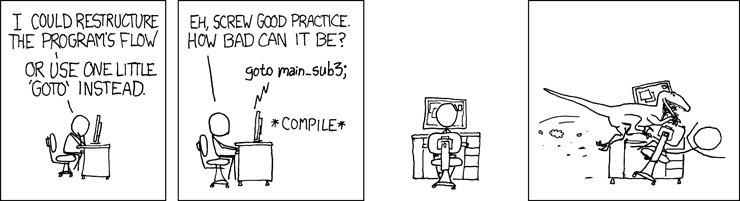
\includegraphics[width=1\textwidth]{figures/document_title_logo.png}
    \end{figure}
    \vfill

    \vspace{1cm}

    \hfill
    \begin{flushright}
        \textbf{\large{Ing. Samuel Lipták}}

        \large{\today}
        % \large{14.06.2024}
    \end{flushright}

\end{center}

\newpage


    \tableofcontents

    % Other pages
    \chapter{New chapter}

    \section{New section}
        Lorem ipsum dolor sit amet, consectetur adipiscing elit \cite{example_citation}. Nullam nec purus

        \subsection{subsection}
            Lorem ipsum dolor sit amet, consectetur adipiscing elit. Nullam nec purus
            \begin{itemize}
                \item Lorem
                \item Lorem
                \item Lorem
            \end{itemize}

        \begin{listing}[!ht]
            \begin{minted}[frame=lines,framesep=2mm,baselinestretch=1.2,fontsize=\footnotesize,linenos]{Python}
print("Hello, world!")
print("This is the placeholder code!")
print("This is the new code!")
# Add your code here
# ...
# ...
# ...
# ...
# ...
# ...
# ...
# ...
# ...
# ...
            \end{minted}
            \caption{Ukážka použitia kódu v dokumente}
        \end{listing}
    % ...

    \newpage
    \listoflistings
    \listoffigures
    \listoftables

    \begin{thebibliography}{1}

	\bibitem{example_citation}
	LIPTÁK, Samuel, 2024. Default-Latex-Document: Source Files. Online. In: Gitlab.com. Available at: \url{https://github.com/Lipetka/default_latex_document}

\end{thebibliography}

\end{document}